\documentclass{beamer}
\usepackage{graphicx}
\usepackage{listings}
\usetheme{metropolis}

\title[WebAssembly]{WebAssembly}
\author{Jakob Waibel}
\institute[Jakob Waibel]{MI7 Druck und Medien}
\date

\begin{document}

\begin{frame}
    \titlepage
\end{frame}

\begin{frame}
    \frametitle{Agenda}
    \tableofcontents
\end{frame}

\section{Einführung}

\begin{frame}{Motivation}
    \begin{figure}
        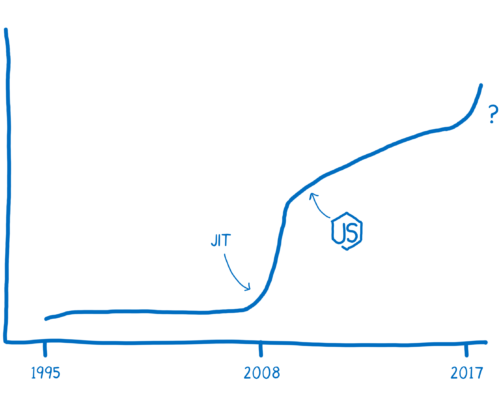
\includegraphics[width=0.7\textwidth,height=0.7\textheight]{./images/perf_history.png}
        \caption{\href{https://hacks.mozilla.org/2017/02/a-cartoon-intro-to-webassembly/}{Performance-Entwicklung im Web-Kontext}}
    \end{figure}
\end{frame}

\begin{frame}{Definition}
    \begin{figure}
        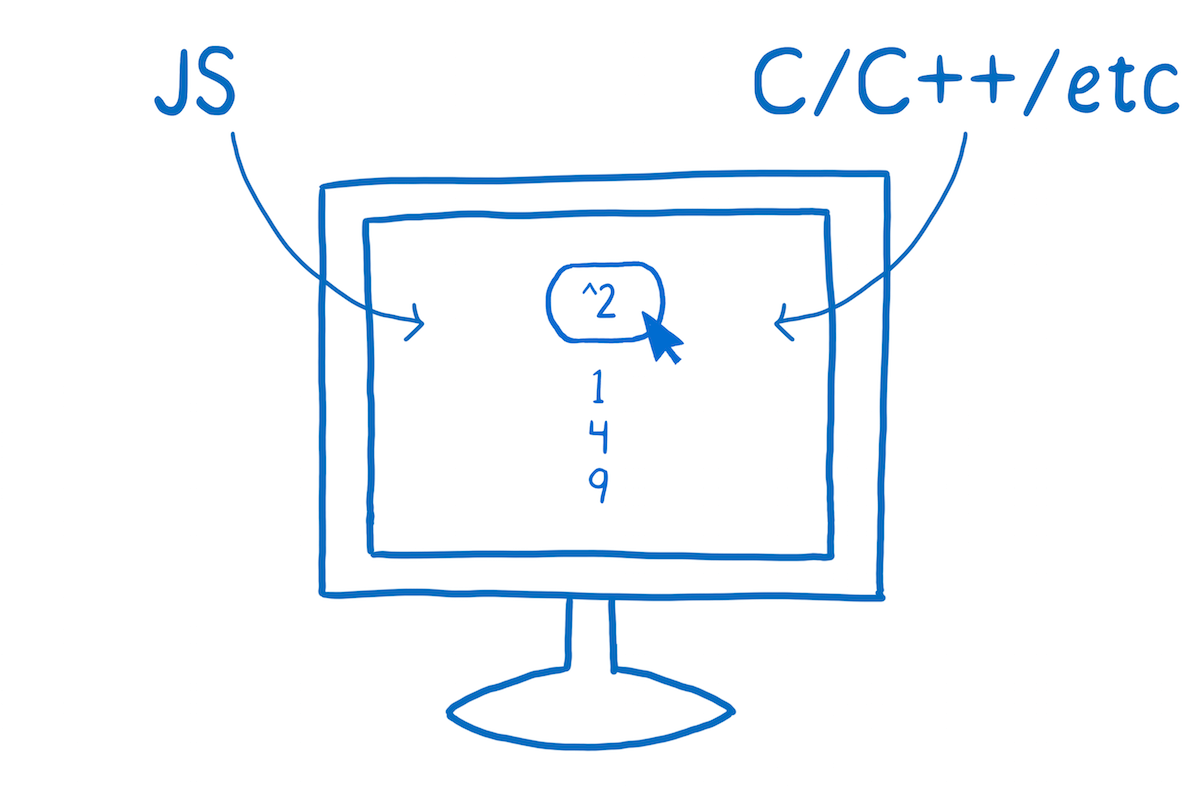
\includegraphics[scale=0.2]{./images/definition.png}
        \caption{\href{https://www.smashingmagazine.com/2017/05/abridged-cartoon-introduction-webassembly/}{Introduction to WebAssembly}}
    \end{figure}
\end{frame}

\begin{frame}{Definition}
    \begin{figure}
        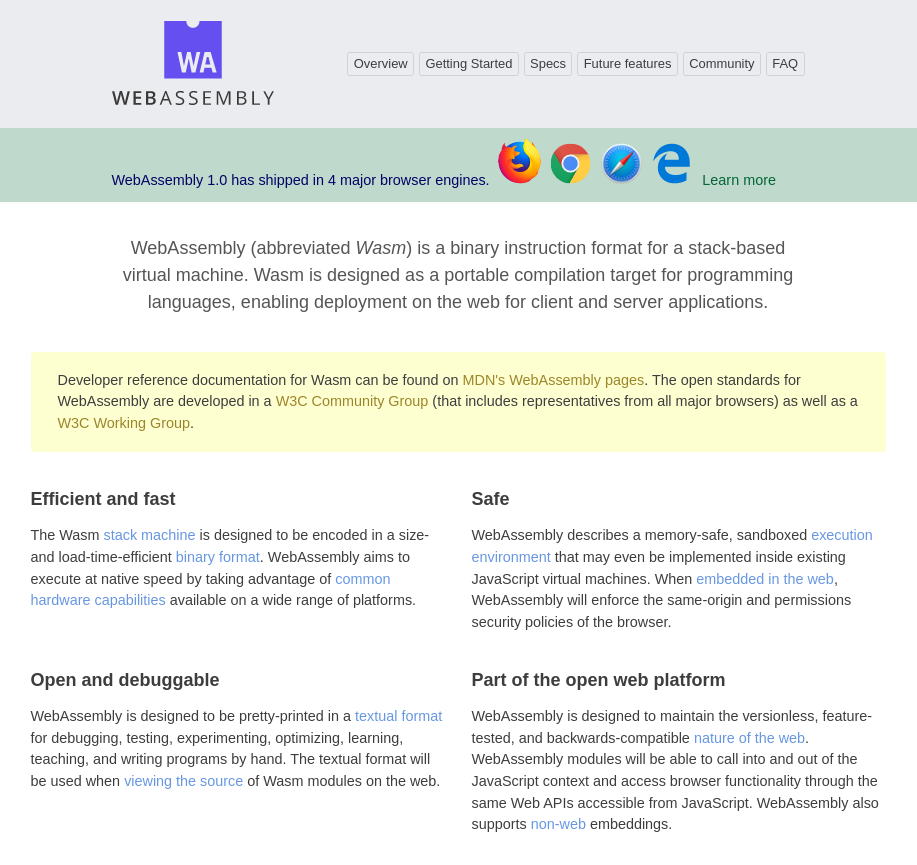
\includegraphics[scale=0.2]{./images/webassembly_org.png}
        \caption{\href{https://webassembly.org/}{webassembly.org}}
    \end{figure}
\end{frame}

\begin{frame}{Definition}
    \begin{quotation}
        "\textbf{WebAssembly} (abbreviated Wasm) is a \textbf{binary instruction format} for a \textbf{stack-based virtual machine}. Wasm is designed as a \textbf{portable compilation target} for programming languages, \textbf{enabling deployment on the web} for client and server applications."
    \end{quotation}
\end{frame}

\begin{frame}{Binary Instruction Format}
    \begin{itemize}
        \item Machine instruction format consisting of \textbf{1s and 0s} that can be directly decoded and \textbf{executed by the CPU}
        \item \textbf{Targeting different instruction set architectures} (ISA) like x86, ARM or RISC-V
        \item WASM uses \textbf{virtual instructions} for a \textbf{conceptual machine}, not a physical one
        \item Think of WASM instruction set as "intersection" of multiple ISAs that can't be mapped directly to one ISA
    \end{itemize}
\end{frame}

\begin{frame}{Stack-Based Virtual Machine}
    \begin{itemize}
        \item Virtual machine which uses stacks to perform oprations
        \item Famous stack-based VMs are the JVM (Java Virtual Machine) and the CLR (Common Language Runtime)
        \item E.g. to add two numbers in a stack-based VM, the program will push the first number to the stack, push the second and then execute some form of the special instruction add, that will pop the first two elements of the stack and replace them with their sum
        \item When the browser translates WASM to the machine code for the machine the browser is running on, it will use registers. Since the WASM specification does not specify registers, it gives the browser more flexibility to use the best register allocation for  that machine
    \end{itemize}
\end{frame}

\begin{frame}{Portable Compilation Target}
    \begin{itemize}
        \item \textbf{WASM is designed to be executable on a variety of operating systems and instruction set architectures, on the Web and off the Web}
        \item Created as an \textbf{open standard} inside the W3C WebAssembly Community Group
        \item \textbf{Requirements} for WASM execution environments:
              \begin{itemize}
                  \item 8-bit Bytes
                  \item Addressable at byte granularity
                  \item Little endian
                  \item \href{https://webassembly.org/docs/portability/}{...}
              \end{itemize}
    \end{itemize}
\end{frame}

\begin{frame}{Deployment on the Web Platform}
    \begin{itemize}
        \item The \textbf{web platform} can be described in two parts
              \begin{itemize}
                  \item A \textbf{VM/Engine} that runs the code, e.g. V8 or SpiderMonkey
                  \item A set of \textbf{Web APIs} that can be called to control browser/device functionality (DOM, WebGL, Web Audio API etc.)
              \end{itemize}
        \item In the past, only JS could be executed in the browser as it was good enough. Today some performance problems occur as we have to run intensive programs like 3D games, VR and AR etc.
        \item The VM can now load an run two types of code: \textbf{JavaScript and WebAssembly}
        \item The different code types \textbf{can call each other}. The WebAssembly JavaScript API wraps exported JavaScript code with JavaScript functions that can be called normally and WebAssembly code can import and synchronously call normal JavaScript functions.
    \end{itemize}
\end{frame}

\begin{frame}{Definition}
    \begin{quotation}
        "\textbf{WebAssembly} (abbreviated Wasm) is a \textbf{binary instruction format} for a \textbf{stack-based virtual machine}. Wasm is designed as a \textbf{portable compilation target} for programming languages, \textbf{enabling deployment on the web} for client and server applications."
    \end{quotation}
\end{frame}

\begin{frame}{Use Cases}
    Considered by the W3C as now more feasable inside the browser:
    \begin{itemize}
        \item Better execution for languages and toolkits that are currently cross-compiled to the Web
        \item VR and AR
        \item Platform simulation / emulation (DOSBox, QEMU, …)
        \item Remote desktop
        \item Games
        \item Cloud IDEs
        \item \href{https://webassembly.org/docs/use-cases/}{...}
    \end{itemize}
    Outside the browser:
    \begin{itemize}
        \item Server-side applications
        \item Game distribution services
        \item Parallel computation across multiple nodes
    \end{itemize}
\end{frame}

\begin{frame}
    Projects using WebAssembly right now:
    \begin{itemize}
        \item Blazor
        \item Autocad
        \item Figma
        \item Jitsi for virtual backgrounds
        \item Zoom for video encoding
        \item \href{https://wasm.continuation-labs.com/d3demo/}{D3wasm}
        \item ...
    \end{itemize}
\end{frame}

% Talk about S-expressions, import, exports, types, globals and shared memory and talk about why it might be not that relevant for the "normal" webdev
\begin{frame}[fragile]{WebAssembly Text}
    \begin{itemize}
        \item Textual representation of the binary format to allow reading and editing by humans
        \item Designed to be exposed in text editors, browser developer tools, etc.
    \end{itemize}
    \begin{lstlisting}[language=Lisp,basicstyle=\footnotesize]
(module
  (func $add (param $lhs i32) (param $rhs i32) (result i32)
    local.get $lhs
    local.get $rhs
    i32.add)
  (export "add" (func $add))
)
    \end{lstlisting}
    \begin{itemize}
        \item .wat files can be compiled to .wasm using the WebAssembly Binary Toolkit (WABT)
        \item For more information, consider visiting the \href{https://developer.mozilla.org/en-US/docs/WebAssembly/Understanding_the_text_format}{MDN Web Docs}
    \end{itemize}
\end{frame}

\begin{frame}{Demo - Prerequisites}
    Disclaimer: This Demo is using the \href{https://go.dev/}{Go} programming language. You don't need any knowledge about Go to follow this Demo. Furthermore, I am using Linux! I can't guarantee, nor do I care, that it works on your Windows machine.

    Installing the Go programming language:
    \begin{itemize}
        \item Please follow \underline{\href{https://go.dev/doc/install}{this}} tutorial
    \end{itemize}

\end{frame}

\begin{frame}[fragile]{Demo - File structure}

    \begin{lstlisting}[language=Bash,basicstyle=\footnotesize]
go/
    assets/
        index.html
        main.wasm
        wasm_exec.js
    cmd/
        server/
            main.go
        wasm/
            main.go
    \end{lstlisting}
\end{frame}

\begin{frame}[fragile]{Demo - main.go}
    \begin{lstlisting}[language=Go,basicstyle=\footnotesize]
package main

import "fmt"

func main() {
	fmt.Println("Hello World!")
}

    \end{lstlisting}
\end{frame}

\begin{frame}[fragile]{Demo - Compilation}
    To compile your main.go to a WebAssembly main.wasm file, execute the following command in the wasm directory:

    \begin{lstlisting}[language=Bash,basicstyle=\footnotesize]
GOOS=js GOARCH=wasm go build -o  ../../assets/main.wasm
    \end{lstlisting}

    You should now be able to locate a \lstinline{main.wasm} file inside your \lstinline{assets} folder.
\end{frame}

\begin{frame}[fragile]{Demo - JavaScript Glue Code}
    Some JavaScript code is needed to import the WebAssembly Module we just created in the Browser. Fortunately, this code comes with every Go installation. So just go ahead and copy the file into your \lstinline{assets} directory:

    \begin{lstlisting}[language=Bash,basicstyle=\footnotesize]
cp "$(go env GOROOT)/misc/wasm/wasm_exec.js" .
\end{lstlisting}
\end{frame}

% The WebAssembly.instantiateStreaming() function compiles and instantiates a WebAssembly module directly from a 
% streamed underlying source. This is the most efficient, optimized way to load wasm code.
\begin{frame}[fragile]{Demo - index.html}
    \begin{lstlisting}[language=html,basicstyle=\footnotesize]
<html>
    <head>
        <meta charset="utf-8"/>
        <script src="wasm_exec.js"></script>
        <script>
            const go = new Go();

            WebAssembly.instantiateStreaming(
                fetch("main.wasm"), go.importObject
            )
            .then((result) => {
                go.run(result.instance);
            })
        </script>
    </head>
    <body></body>
</html>
\end{lstlisting}
\end{frame}

\begin{frame}[fragile]{Demo - cmd/server/main.go}
    \begin{lstlisting}[language=html,basicstyle=\footnotesize]
package main

import (
	"fmt"
	"net/http"
)

func main() {
    err := http.ListenAndServe(
        ":9090", 
        http.FileServer(http.Dir("../../assets"))
    )
    if err != nil {
	fmt.Println("Failed to start server", err)
	return
    }
}

    \end{lstlisting}
\end{frame}

\begin{frame}[fragile]{Demo - Execution}
Now you can run your server and inspect the outcome. Make sure you are in the \lstinline{server} directory, when executing this command:
\begin{lstlisting}[language=bash,basicstyle=\footnotesize]
go run main.go
\end{lstlisting}

Now you should be able to inspect the result in your browser: 
\begin{figure}
    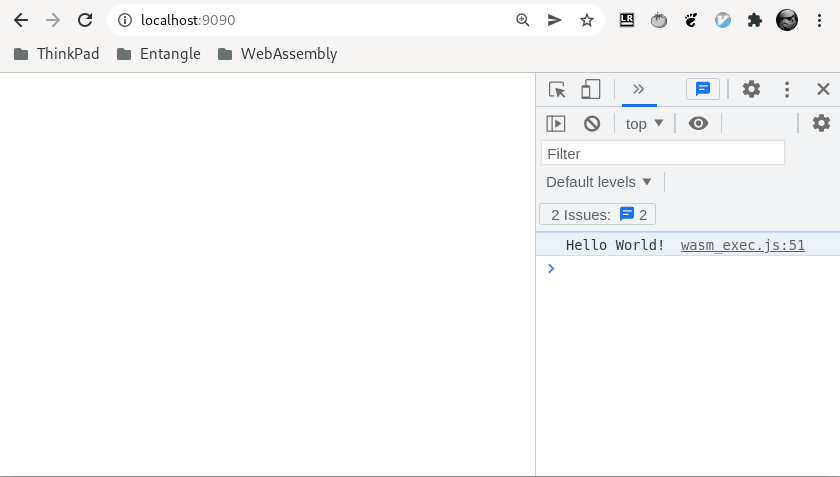
\includegraphics[scale=0.3]{./images/demo.png}
    \caption{\href{https://hacks.mozilla.org/2017/02/a-cartoon-intro-to-webassembly/}{Performance-Entwicklung im Web-Kontext}}
\end{figure}
\end{frame}

\begin{frame}{Demo - Exports}
Essentially same procedure. Just exchange the contents of the following files: 
\begin{figure}
    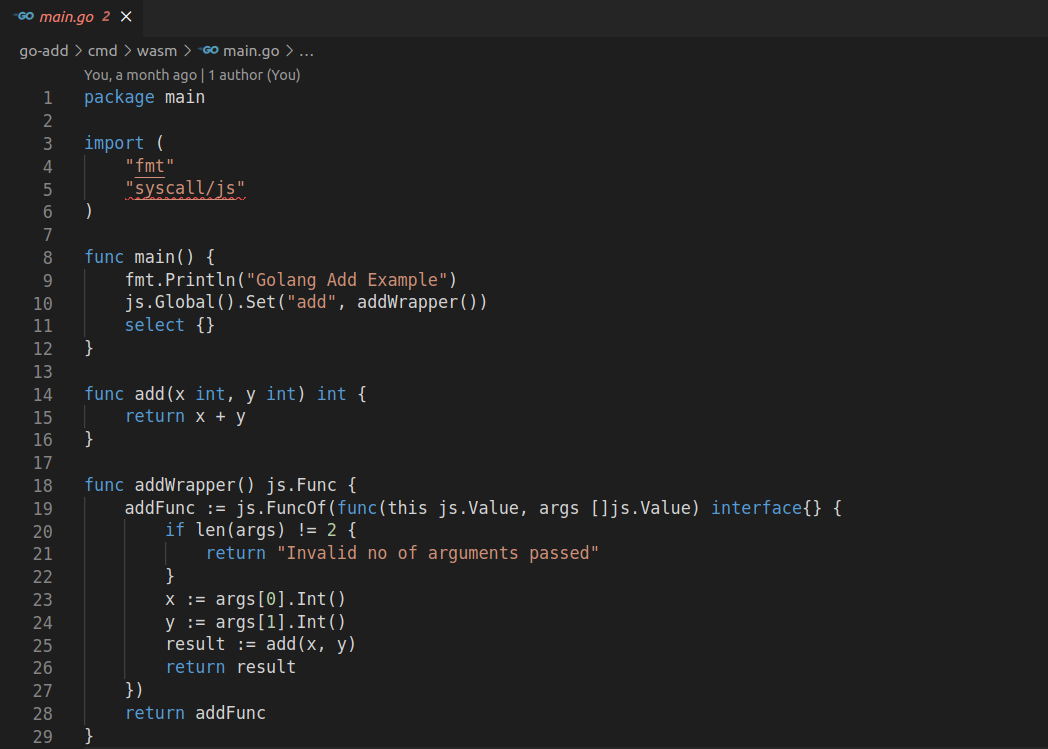
\includegraphics[scale=0.2]{./images/main.png}
    \caption{main.go}
\end{figure}

\end{frame}

\begin{frame}{Demo - Exports}
\begin{figure}
    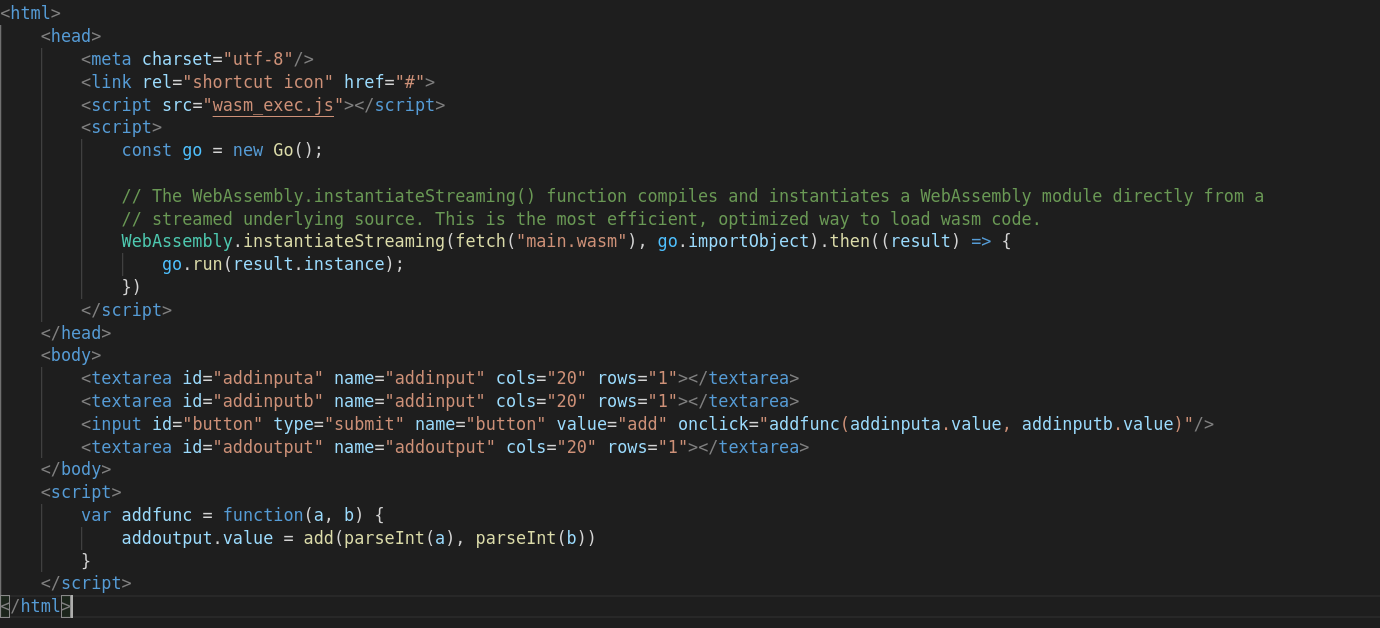
\includegraphics[scale=0.2]{./images/index.png}
    \caption{index.html}
\end{figure}

\end{frame}

\begin{frame}{Demo - Imports}
Essentially same procedure. This time, exchange the contents of the following files: 
\begin{figure}
    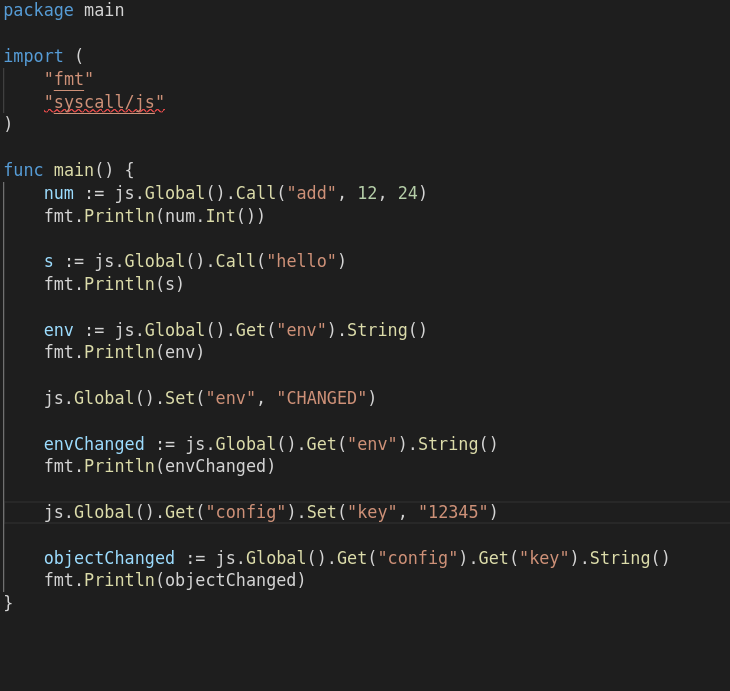
\includegraphics[scale=0.2]{./images/maingo.png}
    \caption{main.go}
\end{figure}

\end{frame}

\begin{frame}{Demo - Imports}
\begin{figure}
    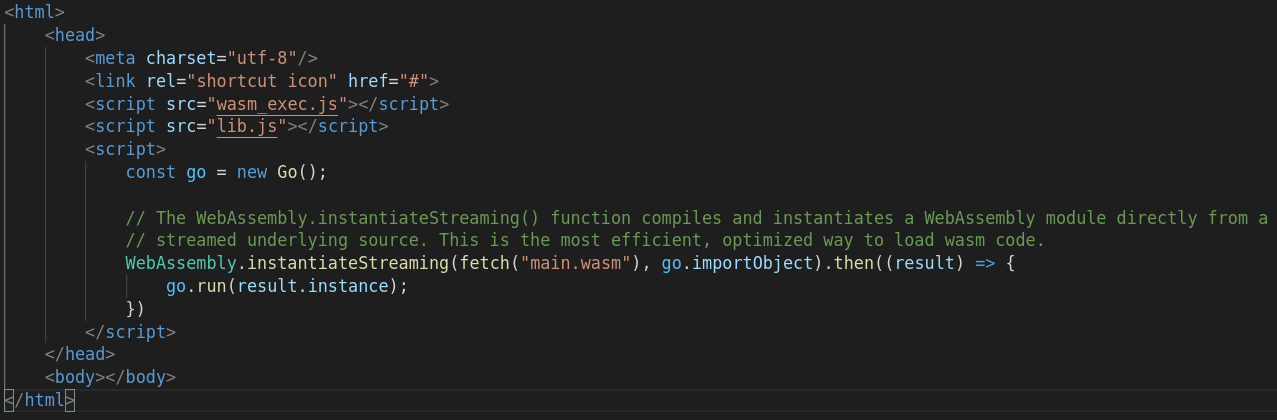
\includegraphics[scale=0.25]{./images/jsindex.png}
    \caption{index.html}
\end{figure}

\end{frame}

\begin{frame}{Demo - Imports}
\begin{figure}
    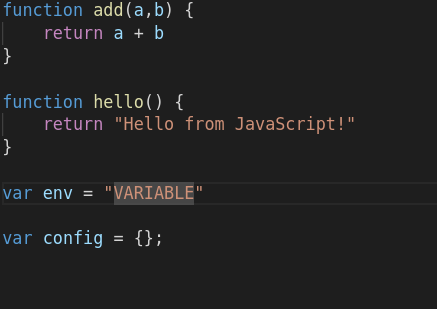
\includegraphics[scale=0.4]{./images/libjs.png}
    \caption{lib.js}
\end{figure}

\end{frame}

\begin{frame}{Additional Information}
\begin{itemize}
    \item Linear Memory - Continuous buffer of unsigned bytes that can be read from and stored into by both Wasm and Javascript
    \item Dom Manipulation - The syscall/js package can also be used to interact with the DOM
    \item E.g. Rust is using wasm-bindgen to achieve the same as Go with syscall/js, AssemblyScript provides those features out of the box...
\end{itemize}
\end{frame}

% Add terminlogy but don't talk about it in the presentation. It should be clear after the Demo
\begin{frame}{Terminology}
\begin{itemize} 
    \item \textbf{Module}: WebAssembly Binary that has beed compiled into executable machine code. A Module is stateless and thus, like a Blob, can be explicitly shared between windows and workers. Module declares imports just like an ES2015 module.
    \item \textbf{Memory}: A resizable ArrayBuffer that contains the linear array of bytes read and written by WebAssembly’s low-level memory access instructions.
    \item \textbf{Table}: A resizable typed array of references (e.g. to functions) that could not otherwise be stored as raw bytes in Memory (for safety and portability reasons).
    \item \textbf{Instance}: A Module paired with all the state it uses at runtime including a Memory, Table, and set of imported values. An Instance is like an ES2015 module that has been loaded into a particular global with a particular set of imports.
\end{itemize}
\end{frame}

\end{document}